\newcommand{\FigMain}[1][t]{
    \begin{figure*}[#1]
        \vskip 0.2in
        \begin{center}
            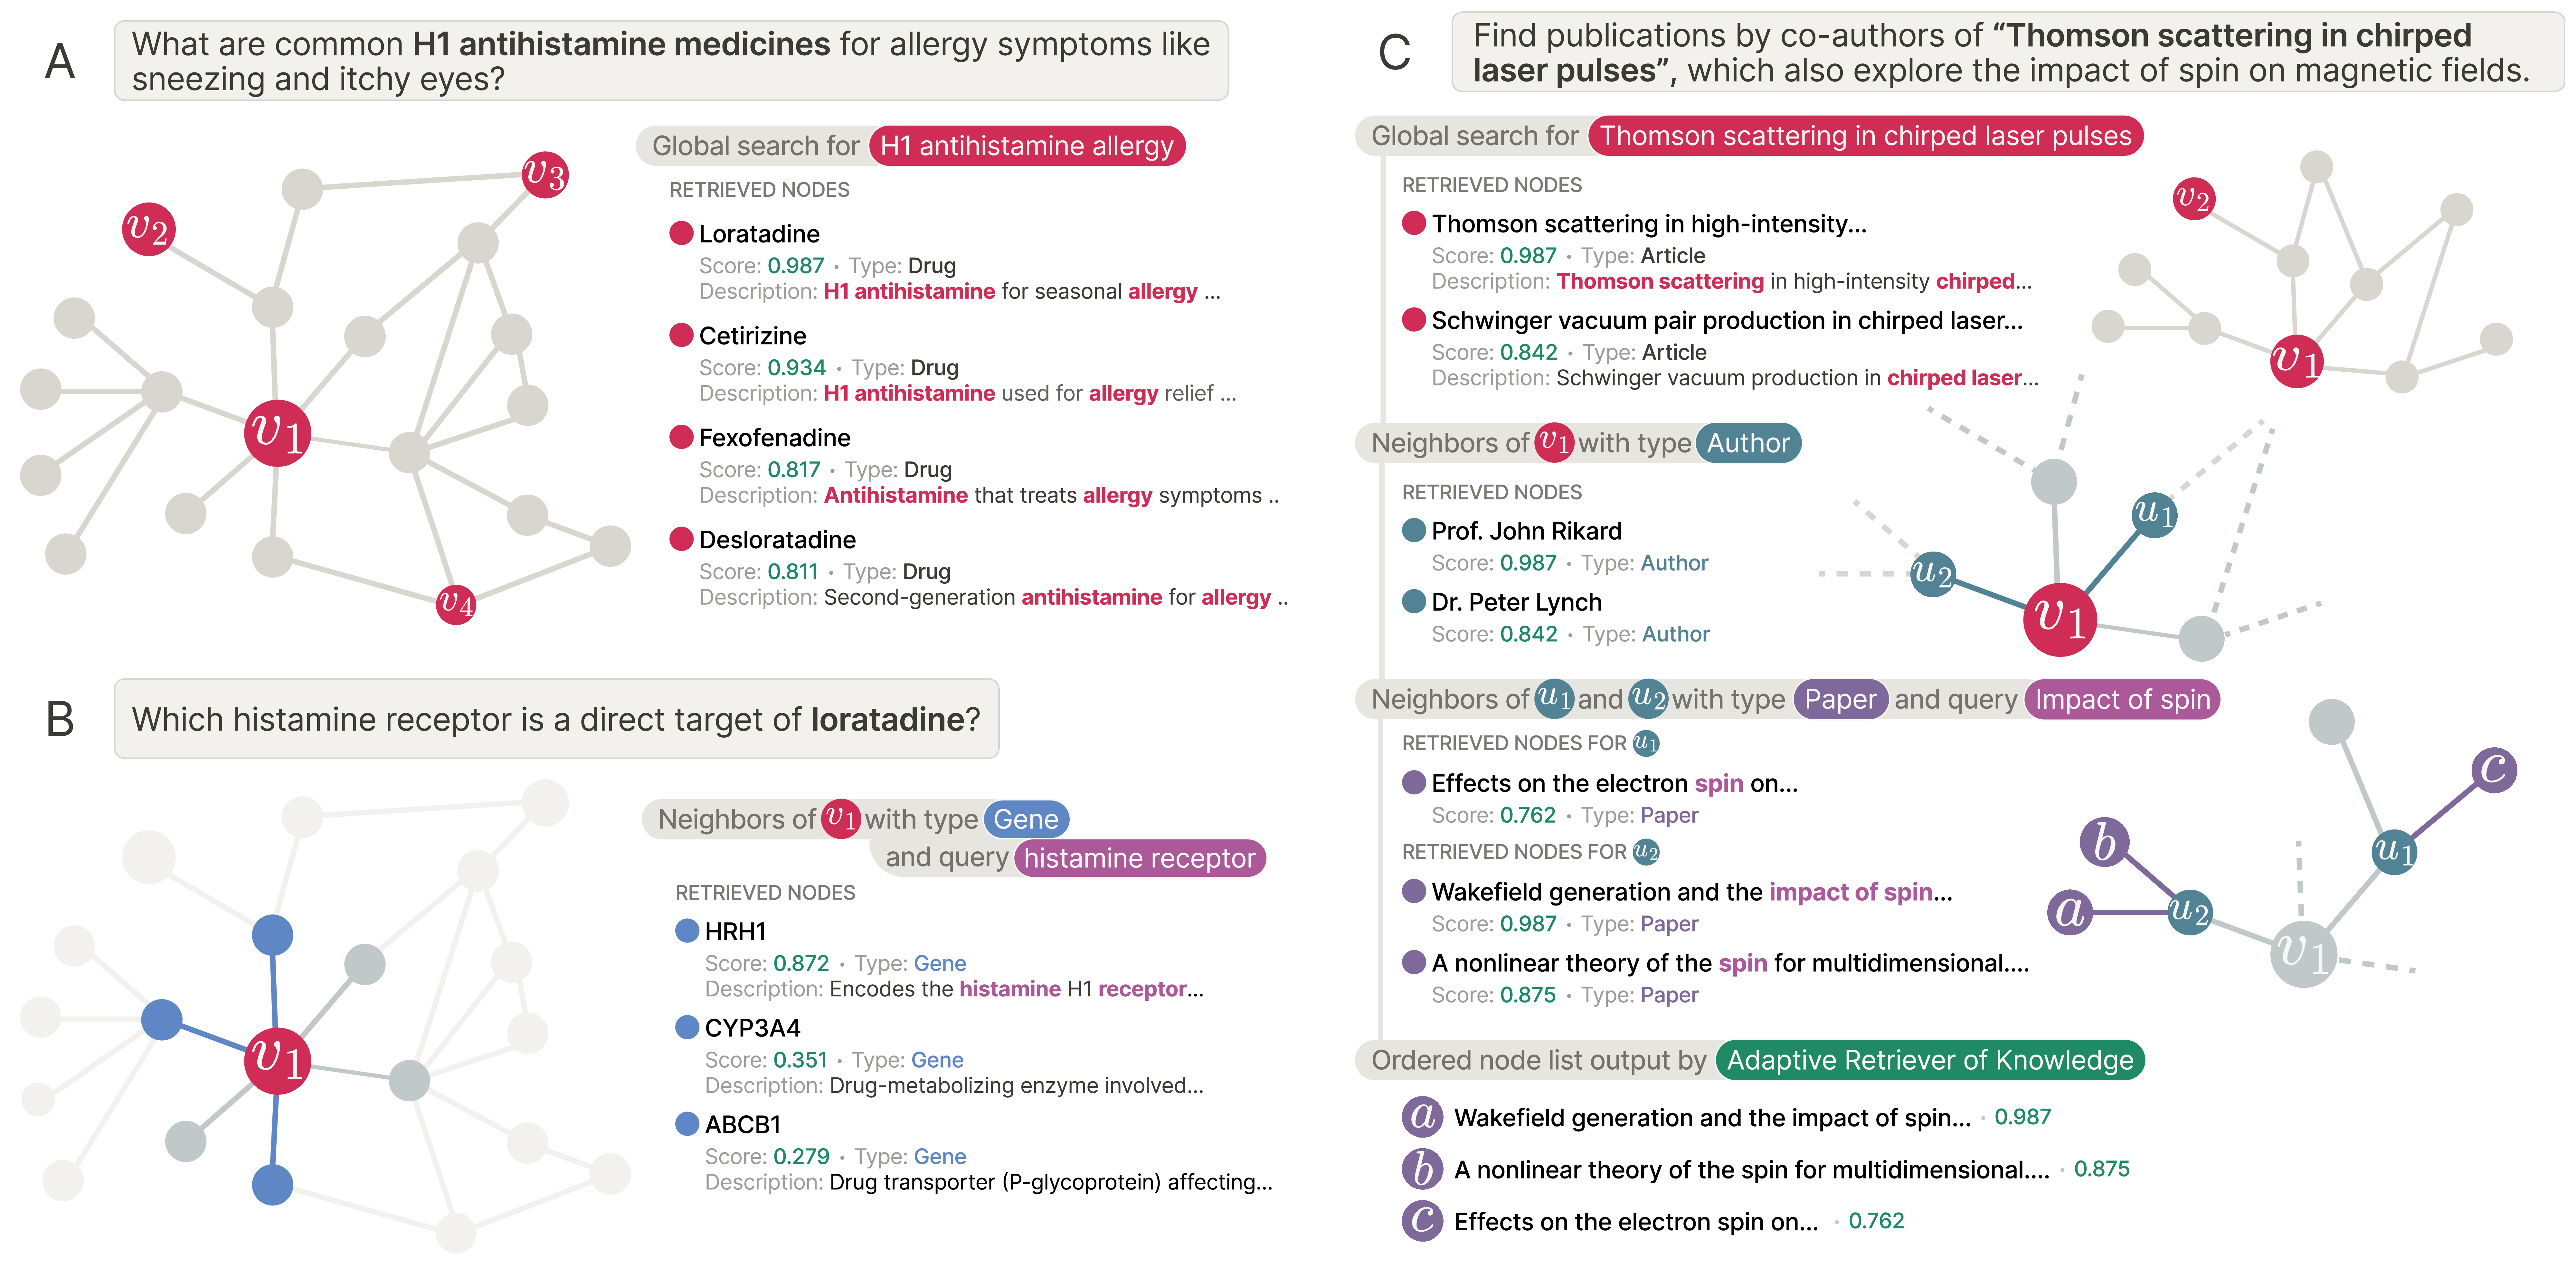
\includegraphics[width=1\textwidth]{./figures/fig-1-main.png}
            \caption{
            Overview of \retriever.
            \retrieverShort interacts with a KG through a minimal two-tool interface:
            \textbf{(a)} For text-dominant queries, \retrieverShort emphasizes breadth by issuing \textsc{Global Search} to retrieve a broad set of candidates.
            \textbf{(b)} For relation-focused queries, \retrieverShort applies \textsc{Neighborhood Exploration} starting from a previously retrieved node (in this case, a drug) and expanding to related entities, enabling targeted relational retrieval.
            \textbf{(c)} For relation-dominant queries, \retrieverShort performs multi-hop retrieval by alternating \textsc{Global Search} and \textsc{Neighborhood Exploration}: it retrieves an initial node (\textit{e.g.}, an article), expands to related entities (\textit{e.g.}, co-authors), and continues expanding and filtering (\textit{e.g.}, papers connected to each author that match query keywords) to recover an ordered set of relevant evidence.
            }
            \label{fig:main-figure}
        \end{center}
        \vskip -0.1in
    \end{figure*}
}

\newcommand{\FigAdaptiveToolUse}[1][t]{
    \begin{figure}[#1]
        \centering
        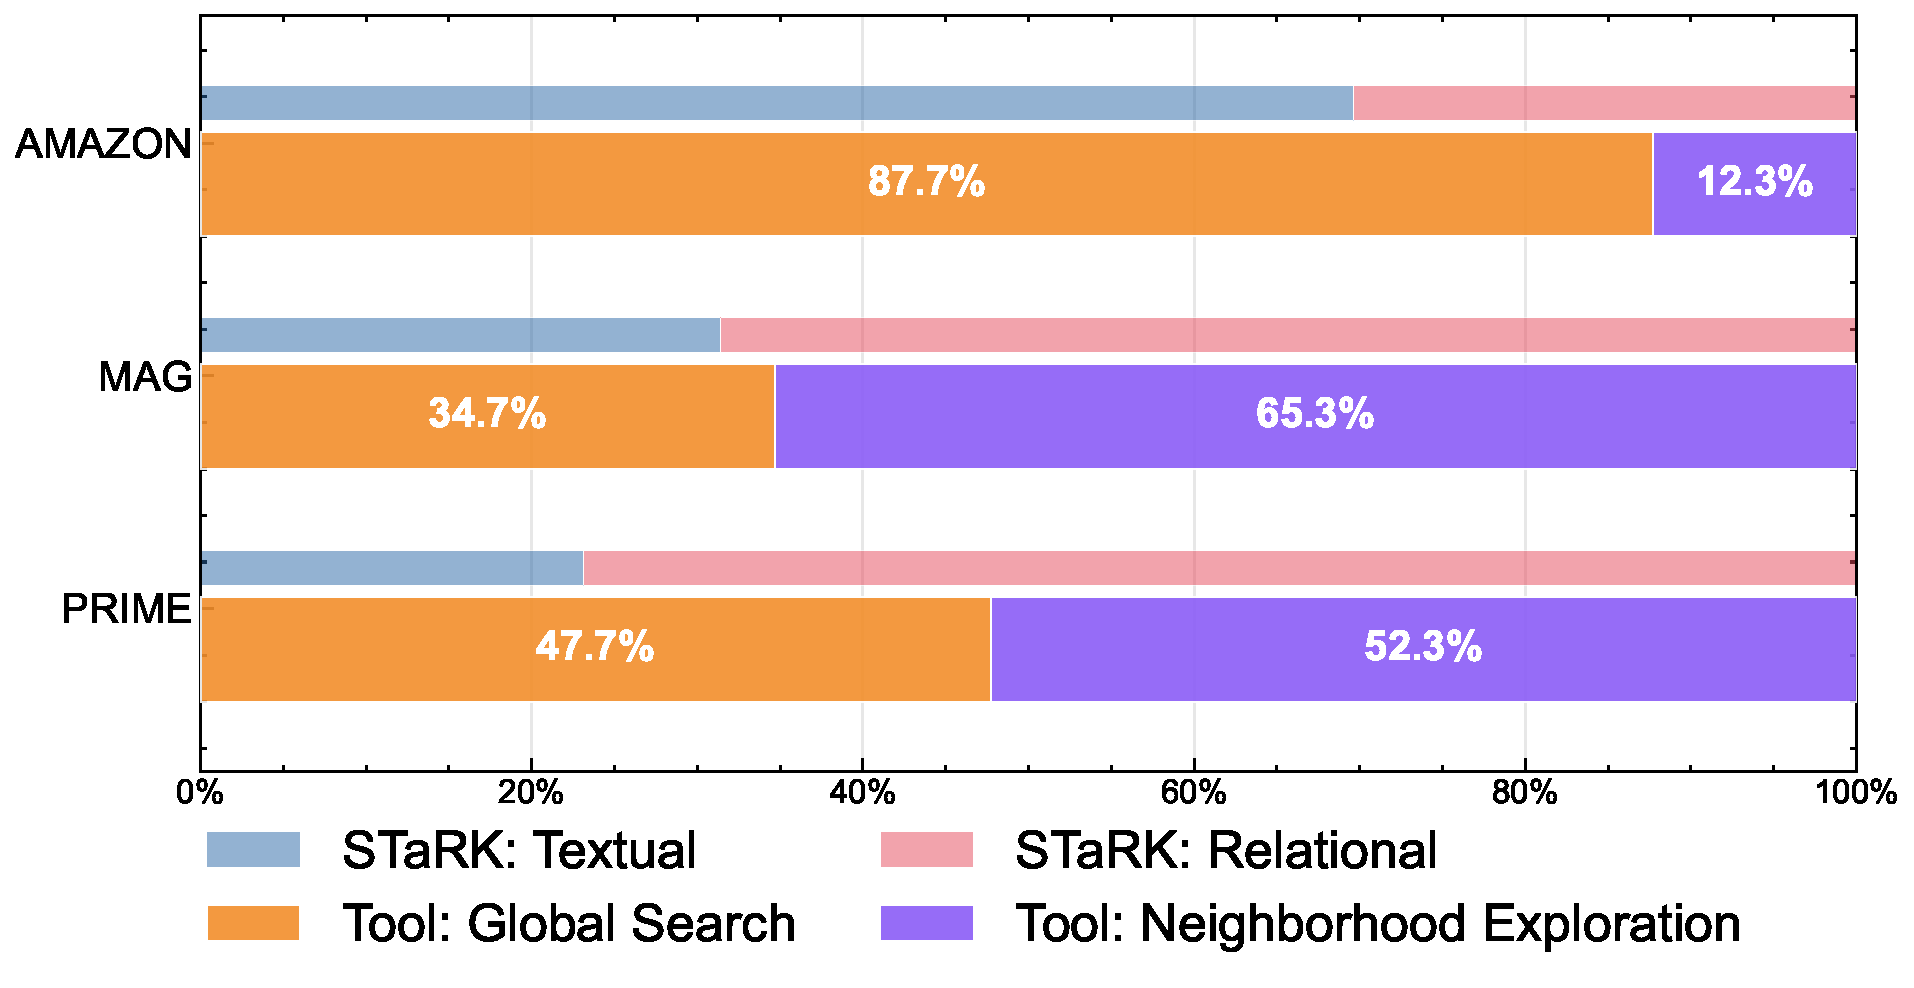
\includegraphics[width=0.48\textwidth]{./figures/fig-3-tool_call_proportions.pdf}
        \caption{
        Thin bars show the share of text- vs.~relation-centric queries in STaRK; thick bars show \retrieverShort's tool-call use. These STaRK annotations are not provided to \retrieverShort; instead, \retrieverShort autonomously shifts tool use to match the dominant query type.
        }
        \label{fig:adaptive-tool-use}
        \vskip -0.2in
    \end{figure}
}

\newcommand{\FigNAgents}[1][t]{
    \begin{figure*}[#1]
        \vskip 0.2in
        \begin{center}
            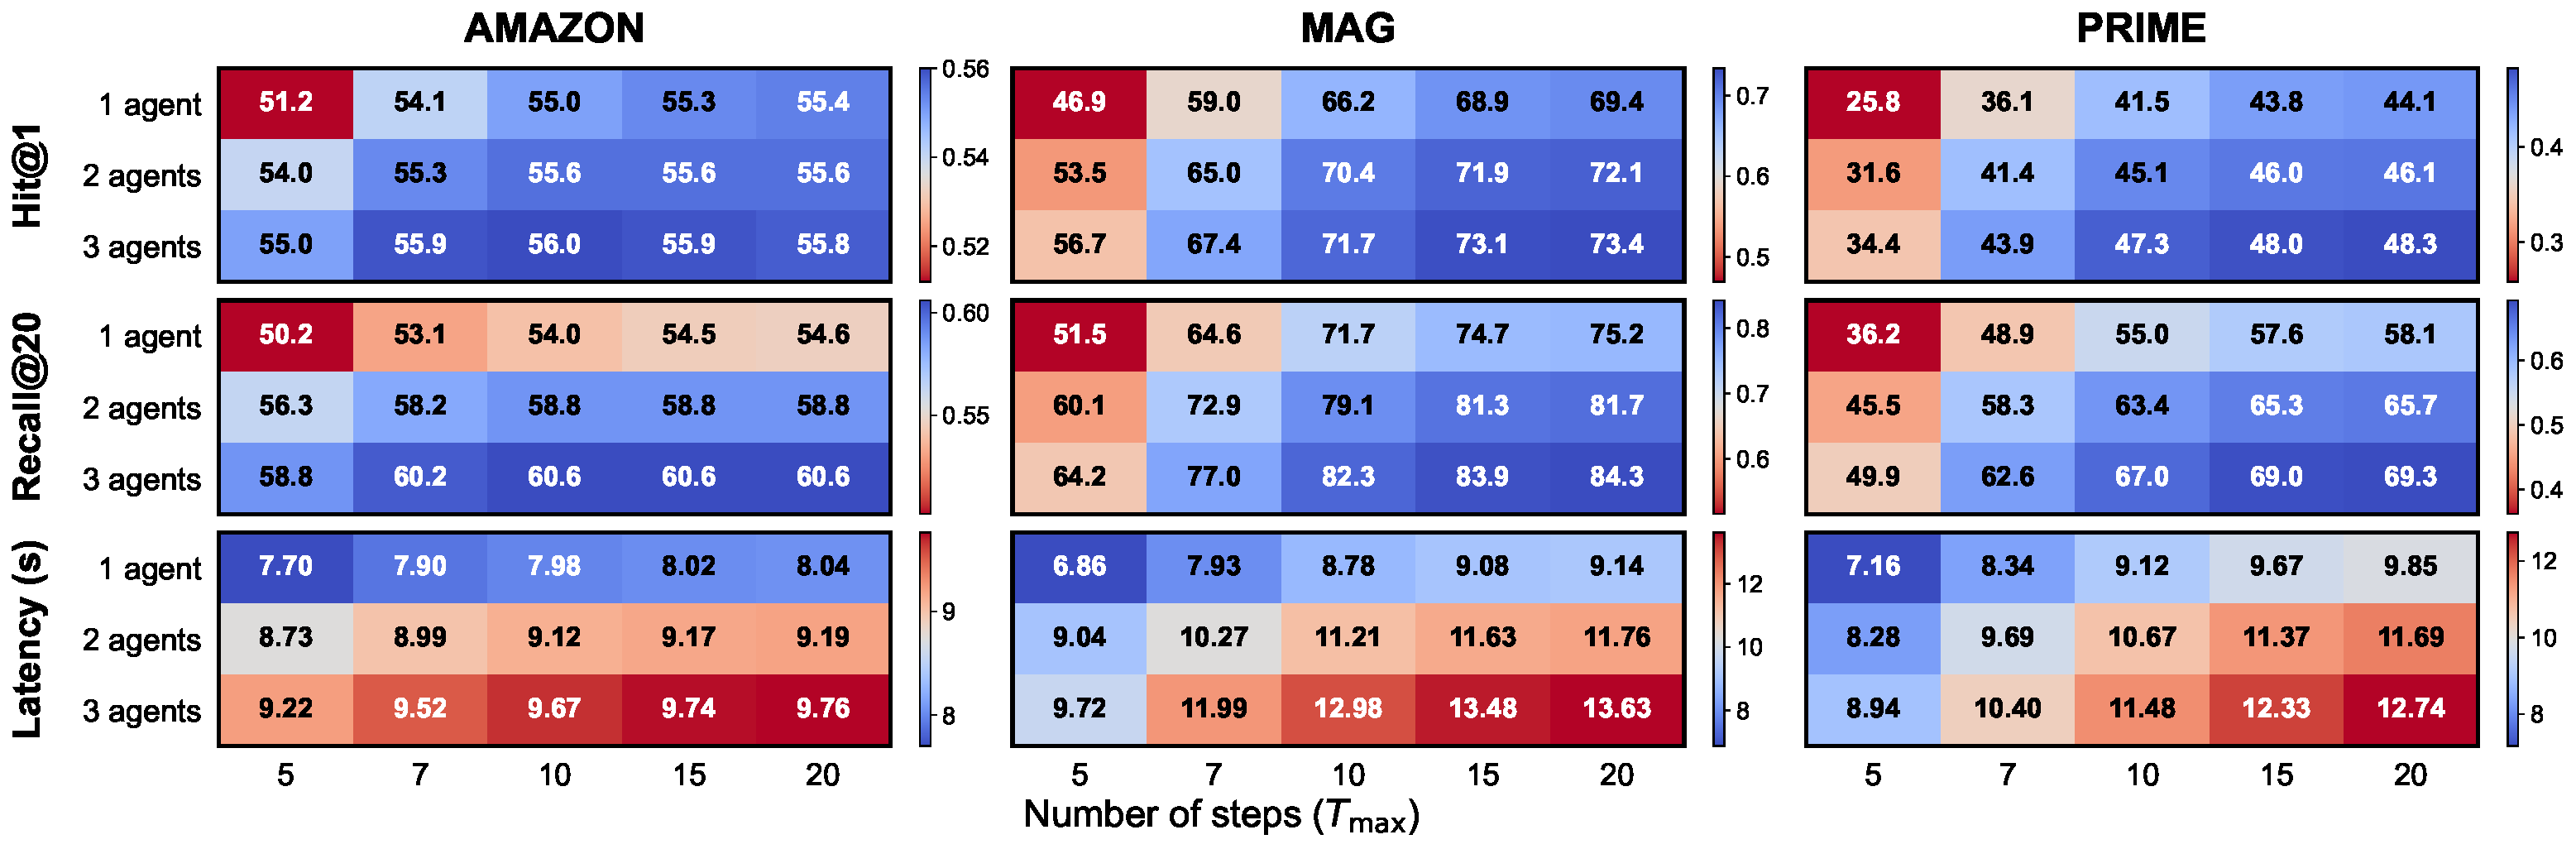
\includegraphics[width=1\textwidth]{./figures/fig-2-compute.pdf}
            \caption{Retrieval quality and latency as a function of inference-time budget. Heatmaps report Hit@1, Recall@20, and end-to-end latency (seconds) on each STaRK graph. Moving from the top left (shallow trajectories, single agent) to the bottom right (deeper trajectories, multi-agent) allocates more compute and improves retrieval performance at the cost of higher latency. Color scales are normalized within each graph and metric for readability.}
            \label{fig:n-agents}
        \end{center}
        \vskip -0.2in
    \end{figure*}
}

\newcommand{\FigSFTImpact}[1][t]{
    \begin{figure*}[#1]
        \begin{center}
            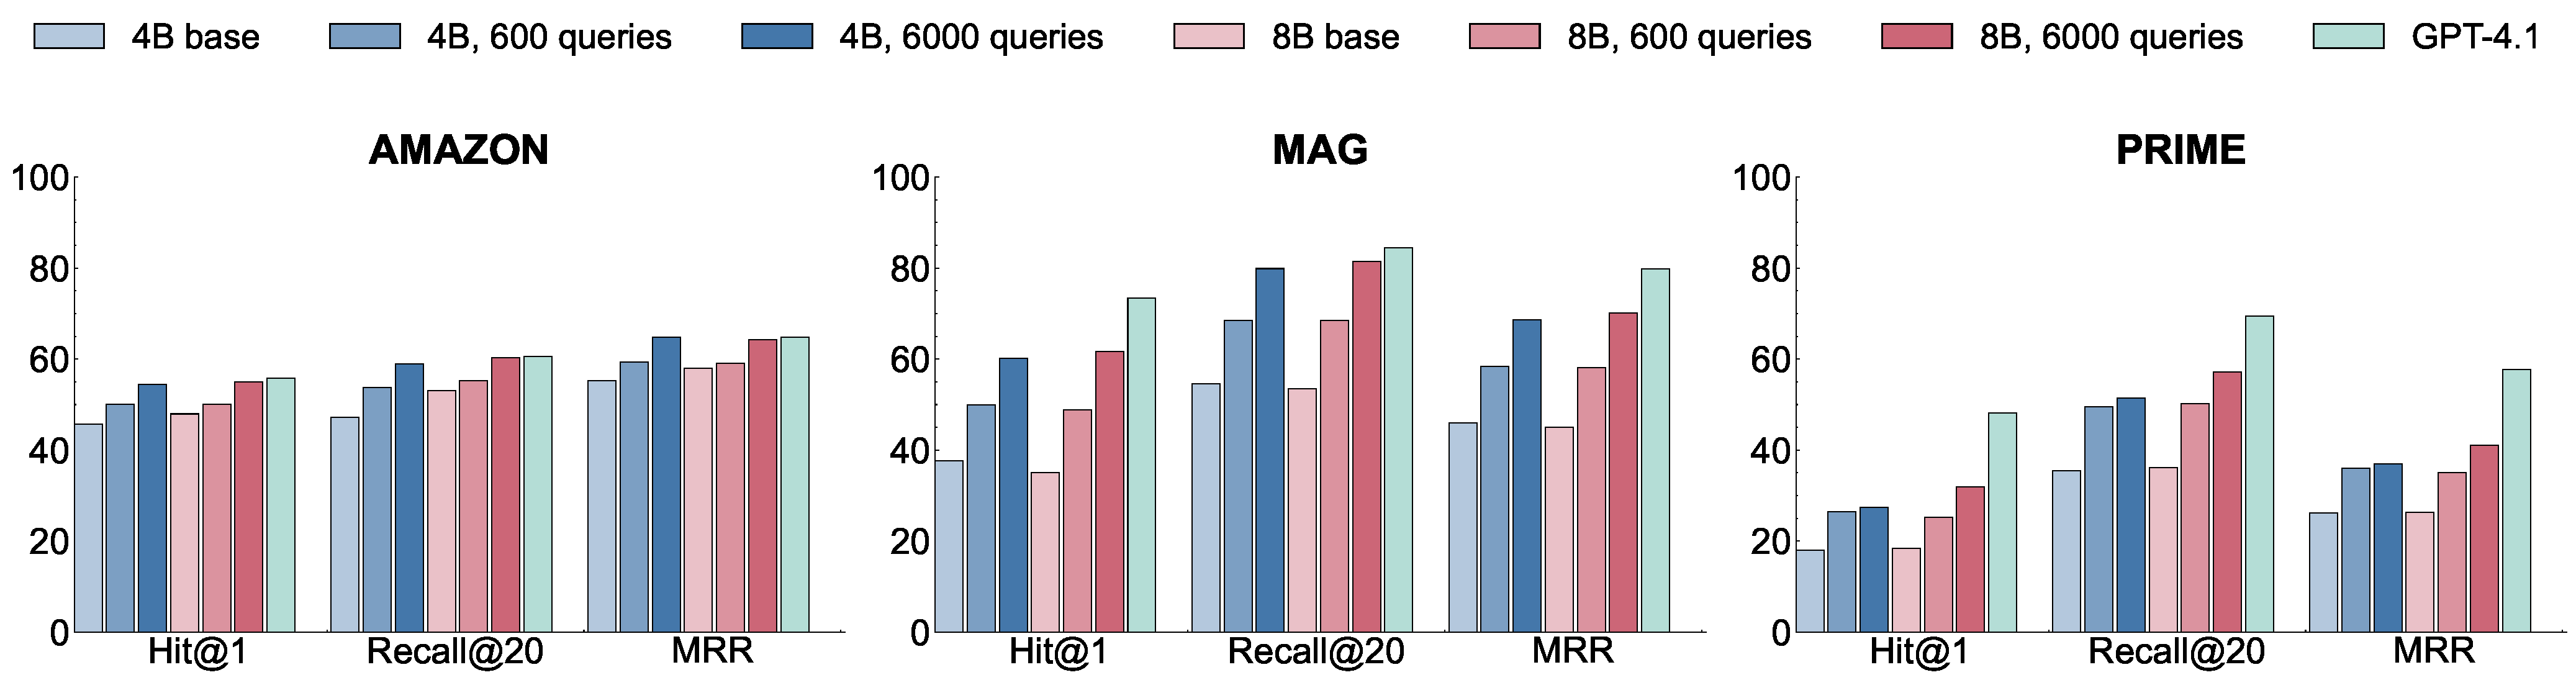
\includegraphics[width=\textwidth]{./figures/fig-4-full_model_comparison_grid.pdf}%
            \caption{Evaluation of the same \retrieverShort pipeline on the STaRK test sets while varying the underlying model and the distillation budget. ``600 queries'' and ``6000 queries'' denote Qwen backbones fine-tuned on trajectories generated by GPT-4.1 from 600 or 6000 training queries per graph, respectively (three trajectories per query; tool calls and observations only; no label supervision).}
            \label{fig:sft-impact}
        \end{center}
    \end{figure*}
}

\newcommand{\FigNeighborExploreDistribution}[1][t]{%
    \begin{figure}[#1]
        \centering
        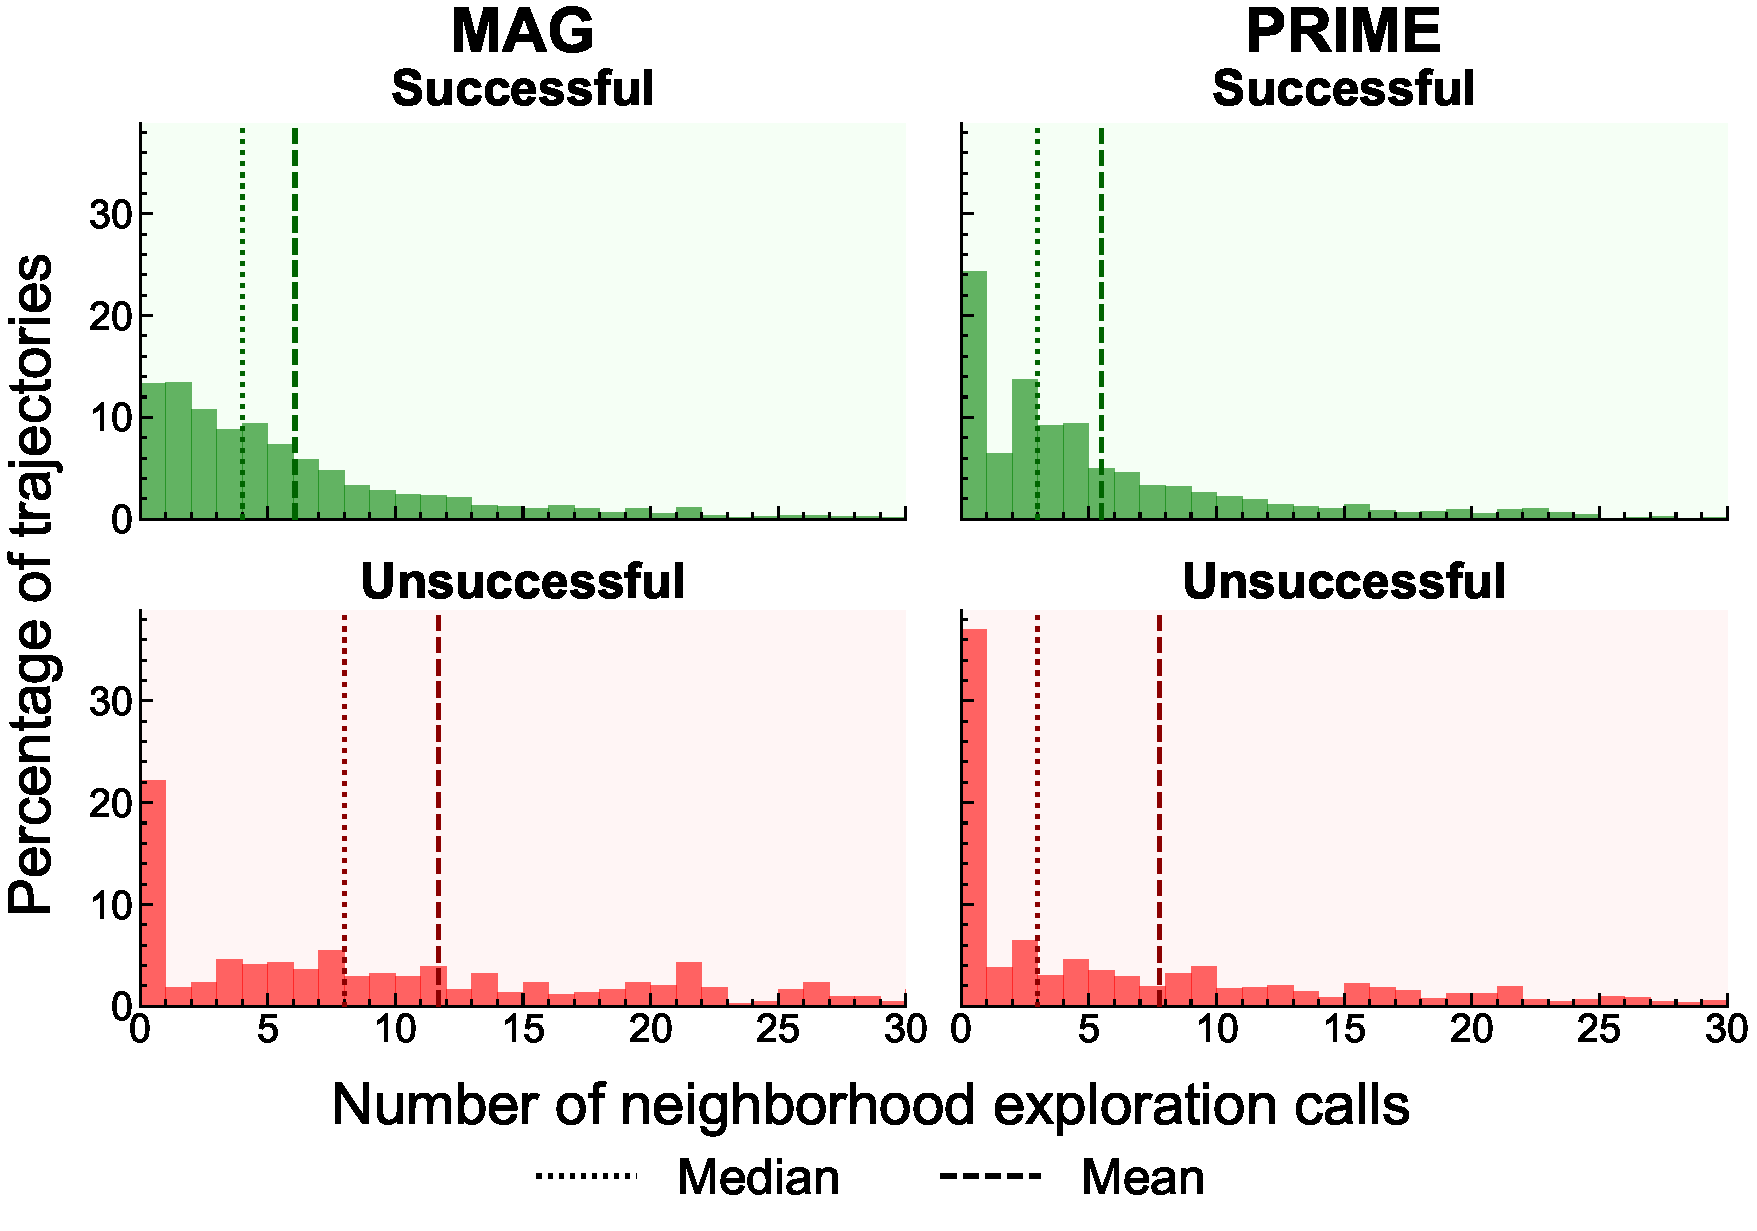
\includegraphics[width=0.48\textwidth]{./figures/fig-5-neighborhood_exploration_tool_calls_distribution.pdf}
        \caption{Distribution of the number of neighborhood exploration calls, split by successful (Hit@5) and unsuccessful trajectories.}
        \label{fig:neighbor-explore-distribution}
        \vskip -0.1in
    \end{figure}
}


\newcommand{\FigArkAgentCli}[1][t]{
    \begin{figure*}[#1]
        \begin{center}
            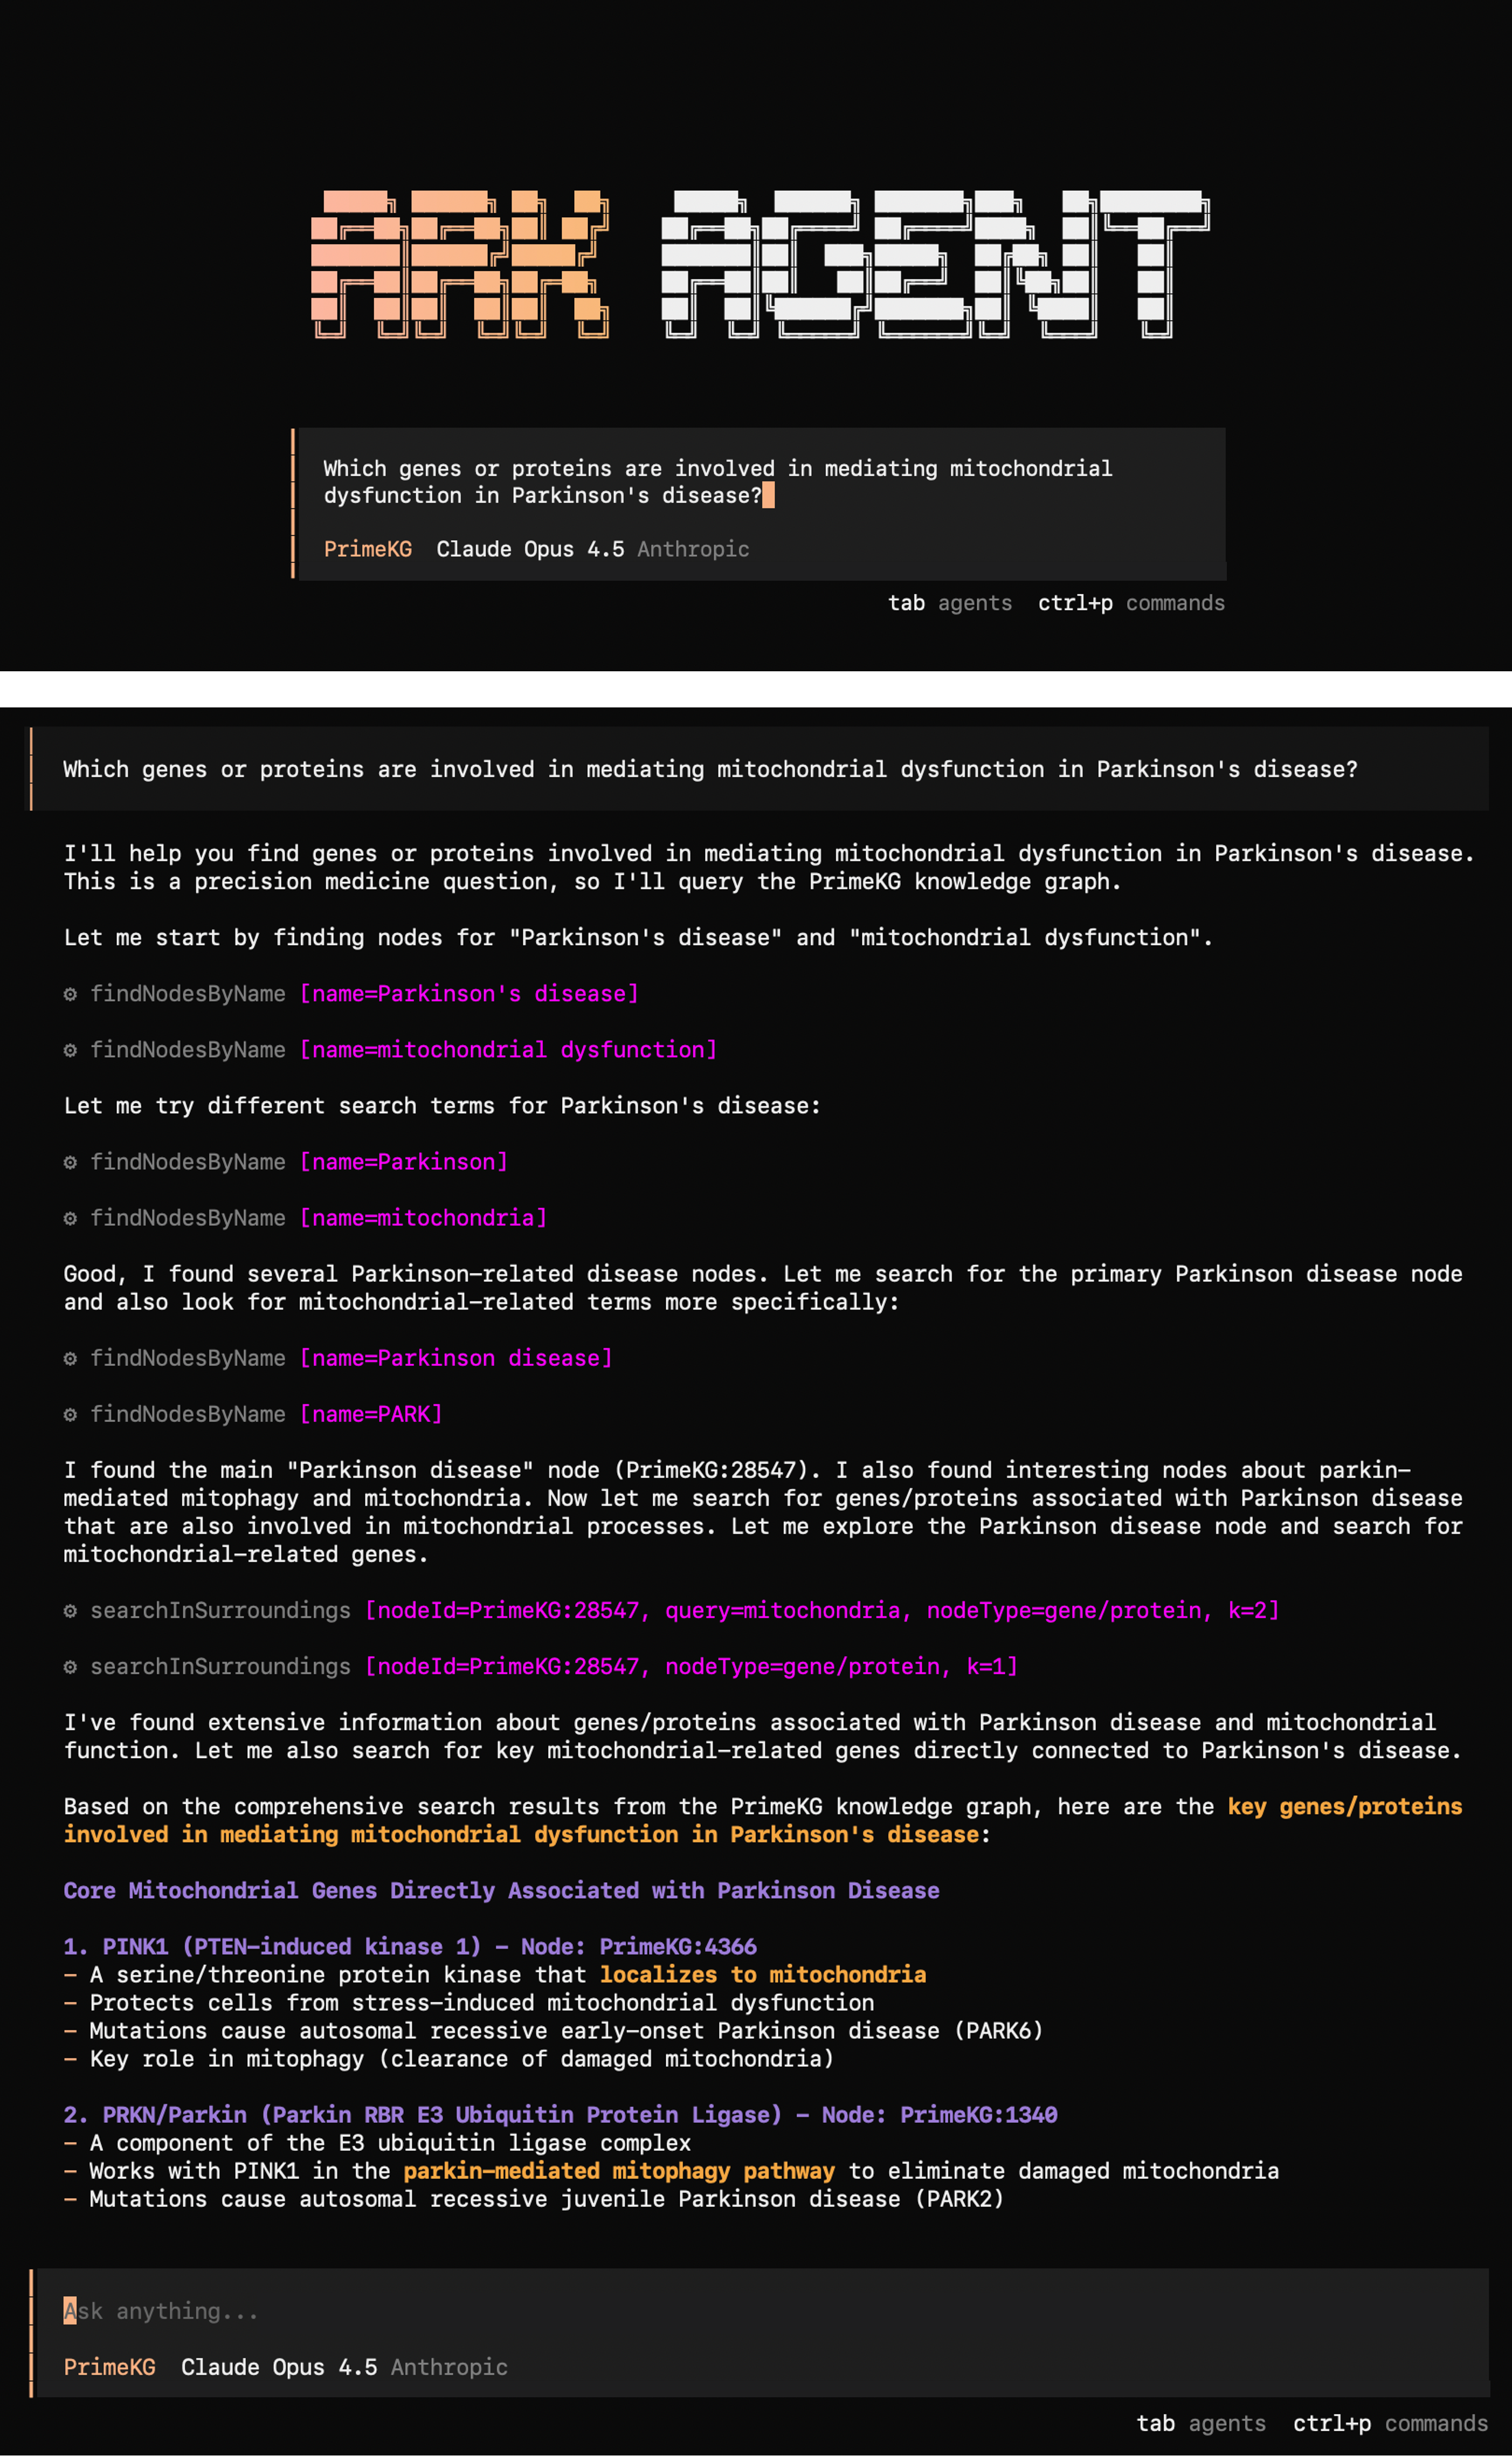
\includegraphics[width=0.9\textwidth]{./figures/fig-a1-ark_agent_cli}
        \caption{Screenshot of the terminal-based chat interface for \retrieverShort, showing query execution and tool use. Given a biomedical query (\textit{e.g.}, ``Which genes or proteins are involved in mediating mitochondrial dysfunction in Parkinson's disease?''), the agent issues global lexical search and neighborhood exploration tool calls to identify relevant nodes in the PrimeKG knowledge graph~\cite{chandak_building_2023}.}
        \label{fig:ark-agent-cli}
        \end{center}
    \end{figure*}
}

